\documentclass[11pt,letterpaper]{article}
\usepackage{naaclhlt2016}
\usepackage{times}
\usepackage{latexsym}
\usepackage{color}

% More packages
\usepackage{amsmath}
\usepackage{amssymb}
\usepackage{framed}
\usepackage{graphicx}
%\usepackage{hyperref}
\usepackage{xspace}

% Some helpful macros
%% Abbreviations
\newcommand{\encdec}{\textsc{EncDec}\xspace}
\newcommand{\attn}{\textsc{AttnBaseline}\xspace}
\newcommand{\attncopy}{\textsc{AttnCopy}\xspace}
\newcommand{\atis}{\textsc{ATIS}\xspace}
\newcommand{\regex}{\textsc{Regex}\xspace}
\newcommand{\geo}{\textsc{Geo}\xspace}

\newcommand{\catroot}{\texttt{\$ROOT}\xspace}
\newcommand{\catquotstr}{\texttt{\$Str}\xspace}
\newcommand{\catint}{\texttt{\$Int}\xspace}
\newcommand{\catstate}{\texttt{\$State}\xspace}
\newcommand{\catstateid}{\texttt{\$StateId}\xspace}
\newcommand{\catriver}{\texttt{\$River}\xspace}
\newcommand{\catcity}{\texttt{\$City}\xspace}

%% Mathematical Notation
\newcommand{\vocabin}{\mathcal{V}^{\text{(in)}}}
\newcommand{\phiin}{\phi^{\text{(in)}}}
\newcommand{\vocabout}{\mathcal{V}^{\text{(out)}}}
\newcommand{\phiout}{\phi^{\text{(out)}}}

%\naaclfinalcopy % Uncomment this line for the final submission
\def\naaclpaperid{***} %  Enter the naacl Paper ID here

% To expand the titlebox for more authors, uncomment
% below and set accordingly.
% \addtolength\titlebox{.5in}    

\newcommand\pl[1]{\textcolor{red}{[PL: #1]}}
\newcommand\rj[1]{\textcolor{blue}{[RJ: #1]}}

% Hide comments, see actual page count
%\newcommand\pl[1]{\iffalse #1 \fi}
%\newcommand\rj[1]{\iffalse #1 \fi}

\newcommand\BibTeX{B{\sc ib}\TeX}


%\title{Recurrent Neural Network Semantic Parsing with Compositional Data Augmentation}
% PL: less clunky
\title{Neural Semantic Parsing with Compositional Data Augmentation}
\author{Robin Jia\\
	    Computer Science Department\\
      Stanford University\\
	    {\tt robinjia@stanford.edu}
	  \And
    Percy Liang\\
    Computer Science Department\\
  	Stanford University\\
  {\tt pliang@cs.stanford.edu}}

\date{}

\begin{document}

\maketitle

\begin{abstract}
Current semantic parsers require complex machinery and
extensive feature engineering to achieve high accuracy.
Recurrent neural network (RNN) models 
provide an appealing alternative to these systems,
as they require less engineering effort and 
have been shown to perform well at a wide range of sequence-to-sequence tasks.
In this work, we present two contributions that
together constitute a practical system for neural semantic parsing.
First, we propose a novel RNN model that allows the parser
to generalize to unseen entities.
In addition, we introduce compositional data augmentation,
a new technique which helps our system to learn
about compositionality from limited amounts of training data.
Our system achieves good accuracy on a variety of semantic parsing tasks,
including new state-of-the-art numbers on the \regex domain.
\end{abstract}

\section{Introduction}
\begin{figure}[t] 
\small
\begin{center} 
  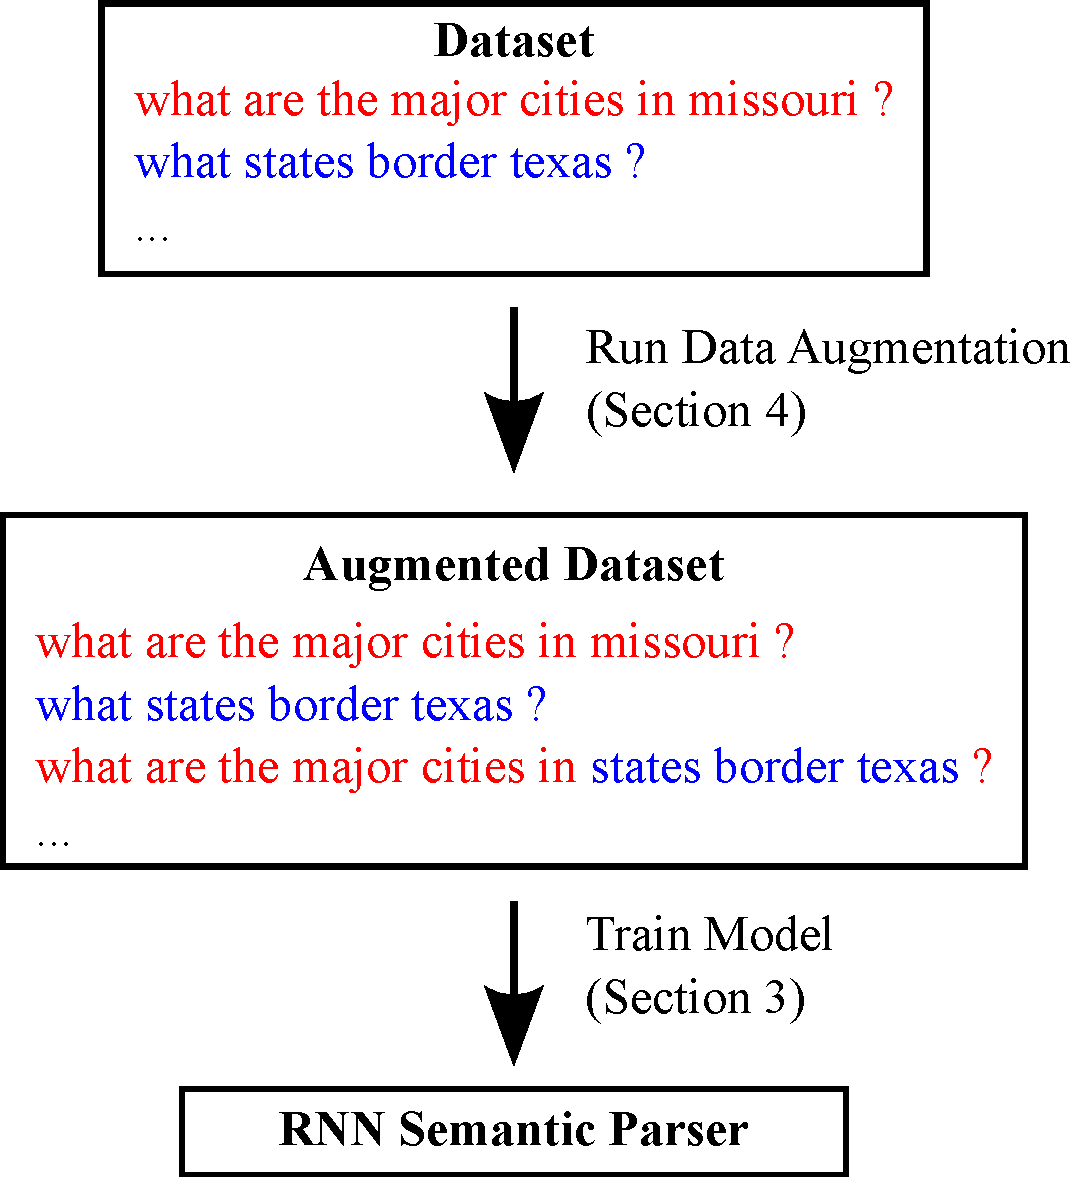
\includegraphics[scale=0.4]{fig-overview.pdf}
\end{center} 
\caption{An overview of our system.
  \rj{What do you think of this?  It's easier to do this figure
    if everything moves down vertically, and I think the colors
  make it clearer what's going on.}
}
\label{fig:overview}
\end{figure}

% Semantic parsing is useful, but complicated
Today, there exist a wide variety of applications that 
require semantic parsing---the precise translation of
natural language utterances into logical forms 
\cite{zelle96geoquery,zettlemoyer05ccg,zettlemoyer07relaxed,liang11dcs,artzi2013weakly,berant2013freebase,kushman2013regex}.
\pl{instead of just saying 'wide variety of applications', say what they are
question answering, robot control, etc. even localizing citations after each application
}
Modern semantic parsers are complex pieces of software
that have a great deal of prior knowledge baked into their internal structure,
and require extensive hand-tuning and domain-specific feature engineering.
Frameworks like CCG must deal with complex lambda calculus expressions,
and systems like SEMPRE \cite{berant2013freebase}
require large amounts of code that define the parser's grammar and features.
% TODO: argue this better

% Comment about our model being general-purpose, maybe delete
%Some recent work has tried to make semantic parsing
%into a general purpose technology \cite{wang2015overnight},
%but the accuracy of these systems leaves much to be desired.
%\pl{the main complaint should be about complexity, not accuracy,
%since in the end, we don't really gain on that}
%\rj{The idea of this sentence was to foreshadow improvements on overnight.
%I'll take it out if we wind up not running those experiments.}
%\pl{in general, use 'accuracy' rather than 'performance' since it's more precise;
%systems people use performance to talk about speed}

% RNNs are great!
RNN models have achieved impressive results on a variety of 
sequence-to-sequence tasks, such as
machine translation \cite{sutskever2014sequence,bahdanau2014neural}, 
syntactic parsing \cite{vinyals2015grammar}, and 
computing convex hulls \cite{vinyals2015pointer}.
RNNs are also appealing for their simplicity, as they require 
little hand-engineering of features.
Even though RNNs generate their output in a linear fashion,
work on syntactic parsing has demonstrated that they can learn
to generate linearized representations of tree-structured outputs as well
\cite{vinayls2015grammar}.

% Datasets small, RNNs don't have built in compositionality
The drawback of these RNN models is that they require
large amounts of data to achieve good accuracy.
LIST NUMBERS OF EXAMPLES.
Meanwhile, semantic parsing datasets often consist of only 
hundreds of labeled examples.
This limited amount of training data
creates two major barriers to applying RNNs to semantic parsing.
First, semantic parsers must be able to generalize to a large set of 
domain-specific entities which, due to the limited
amount of training data, may occur rarely or not at all
in the training dataset.
Second, RNNs do not intrinsically have a notion of compositionality;
in contrast, most semantic parsers have a built-in notion of
hard alignments between fragments of utterances and logical forms
\cite{zettlemoyer05ccg,berant2013freebase},
which helps them generalize at test time.
RNNs can only learn about compositionality through observations of the data.

\pl{be careful - I think we need to explain what we mean by 'compositionality'}
\pl{in general, can tighten this paragraph;
somehow the 'datasets are small, models are generic' message needs to come out more}
\pl{I'd carve up the two problems as follows:
  (i) handle unseen entities (need to explain this with concrete example, ideally in Figure 1);
(ii) handle compositionality (need to explain this more, referencing example in Figure 1)}

% RNN model (handle unseen entities?), data augmentation (handle compositionality?)
In this paper, we present the first (to our knowledge)
semantic parser that uses a sequence-to-sequence RNN model to generate
logical forms.  
The closest related work of which we are aware is
by Grefenstette et al.~\shortcite{grefenstette2014deep};
however, their model was not a sequence-to-sequence model,
and they had yet to achieve good results.
\rj{Here-ish?  Need to transition better.  Alternatively, move to discussion?}
Our contributions are two-fold:
First, we introduce an attention-based copying mechanism 
that allows our RNN sequence-to-sequence model to generalize to unseen entities.
Second, to teach the model about compositionality,
we introduce compositional data augmentation,
which induces a high-precision grammar from the training data
and augments the training data with synthetic examples sampled from this grammar.

%\pl{
%Overall good - flows well and well-motivated, generally like the writing style.
%Currently, you do a good job of giving background about RNNs
%and the challenges that arise when applying to semnatic parsing.
%But the main thing that you need to do more of is highlight our contributions
%and connect it directly with challenges.
%Make it really crisp - don't go for subtlety here: for example,
%say there are two challenges, A, and B.  We tackle A using C and B using D.
%Make our contributions sound as exciting as the challenges!
%}


\section{Task}
We model semantic parsing as a generic sequence-to-sequence task.
The input utterance $x$ is represented as a sequence of words $x_1, \dotsc, x_m
\in \vocabin$, the input vocabulary;
similarly, the output logical form $y$ is represented
as a sequence of tokens $y_1, \dotsc, y_n \in \vocabout$, the output vocabulary.
A linear sequence of tokens might appear to lose the hierarchical structure of a logical form,
%instead of an abstract syntax tree may seem unnatural,
%but this choice makes it easier to define our RNN model.
but there is precedent: \newcite{vinyals2015grammar}
showed that RNNs can reliably predict tree-structured outputs
in a linear fashion for syntactic parsing.
Figure FIG shows example input-output pairs for the different
datasets used in this paper.
% TODO: make this figure

\pl{need FIGURE with a concrete example}

\subsection{Datasets}
%\begin{table}[t]
%  \centering
%  \small
%  \begin{tabular}{|l|c|c|c|}
%    \hline
%    Dataset & Training Examples & Test Examples \\
%    \hline
%    \atis & 4473 & 448 \\
%    \regex & 660 & 164 \\
%    \geo & 600 & 280 \\
%    \hline
%  \end{tabular}
%  \caption{Overview of the datasets used in this paper.  
%  Note that For \regex, we create our own split by randomly partitioning the dataset.}
%  \label{tab:datasets}
%\end{table}

We evaluate our system on three standard semantic parsing datasets:
\begin{itemize}
  \item \textbf{ATIS} (\atis) contains 
    natural language queries for an flights database
    paired with corresponding database queries written in a 
    lambda calculus-based language.  
    We train on $4473$ examples and evaluate on the $448$
    test examples used by Zettlemoyer and 
    Collins~\shortcite{zettlemoyer07relaxed}.

  \item \textbf{Regular Expressions} (\regex)
  contains natural language descriptions of regular expressions
  paired with associated regular expressions.
  Unlike Kushman and Barzilay~\shortcite{kushman2013regex}, 
  we primarily evaluate
  on a test set of $164$ examples we selected randomly
  from the dataset;
  however, to compare with their results, we also evaluate
  with 3-fold cross-validation.

  \item \textbf{GeoQuery} (\geo) contains
  natural language questions about US geography
  paired with corresponding database queries written in a Prolog-based
  query language.
  We use the 600/280 split first used by
  Zetlemoyer and Collins~\shortcite{zettlemoyer05ccg}.
\end{itemize}

It is notable that these datasets are many orders of magnitude smaller
than those used to train neural machine translation systems
\cite{sutskever2014sequence,bahdanau2014neural}.

In this work, we only explore learning from logical forms.
We therefore do not use any semantic parsing datasets
that only include denotations,
such as \textsc{WebQuestions} \cite{berant2013freebase}.
We discuss the possibility of learning from denotations
in Section~\ref{sec:discussion}.

%\pl{no intrinsic reason why we can't have denotations;
%state in a more neutral way}

\section{RNN Model}
\begin{figure}[t] 
\small
\begin{center} 
  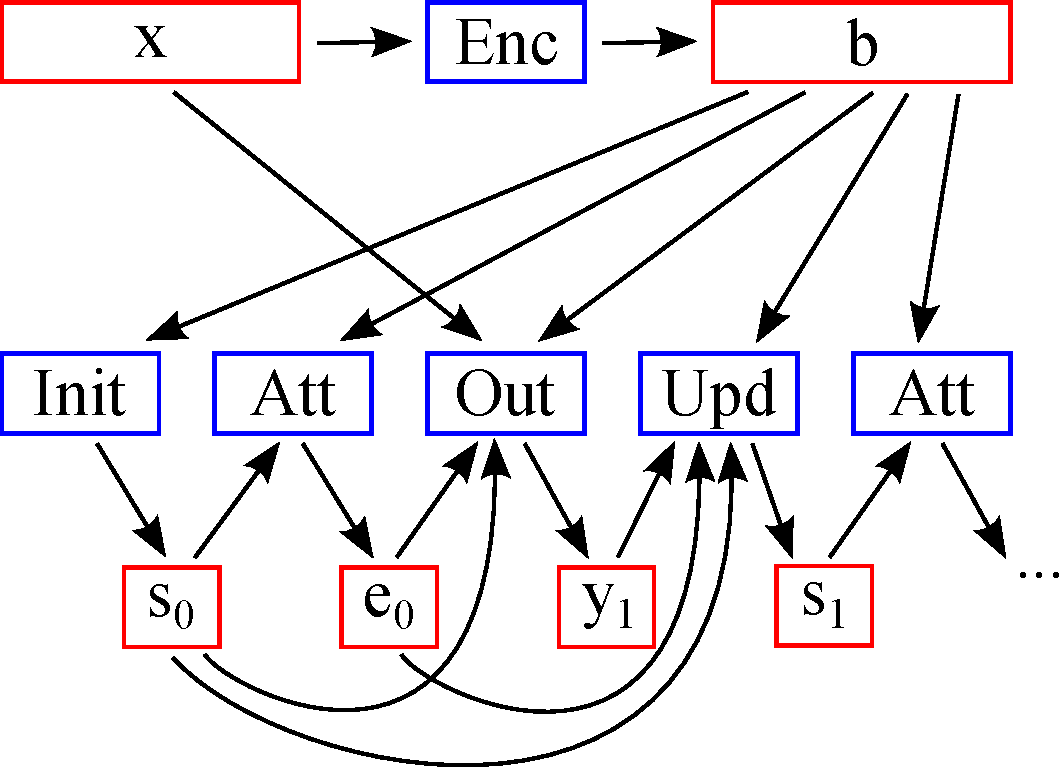
\includegraphics[scale=0.4]{fig-rnn.pdf}
\end{center} 
\caption{An overview of our RNN model.  
  Enc, Encoder; Init, Decoder Initialization;
  Att, Decoder Attention; Out, Decoder Output;
  Upd; Decoder Update.
}
\label{fig:rnn}
\end{figure}
Our neural semantic parser is backed by a generic sequence-to-sequence RNN model.
This model is based closely on existing 
attention-based neural machine translation models
\cite{luong2015translation},
but also includes a novel attention-based copying mechanism.

\pl{we should have a paragraph after our description
  or in discussion comparing our model with neural MT models;
  doing a careful diff is important }
  \rj{It's basically the same as Thang's other than the output module}

At a high level, our system consists of two main modules:
\begin{enumerate}
  \item \textbf{Encoder Module}.  This module 
    converts the input sequence $x_1, \dotsc, x_m$
    into a sequence of context-sensitive embeddings
    $b_1, \dotsc, b_m$,
    where each $b_i$ is a real-valued fixed-dimensional vector.
  \item \textbf{Decoder Module}.  This module
    takes in the input sequence and annotations,
    and generates a probability distribution
    over sequences $y = y_1, \dotsc, y_n$,
    where each $y_j \in \vocabout$.
    It writes the output tokens one at a time,
    maintaining a hidden state $s_j$ at each time $j$.
    It generates the next output token $y_{j+1}$ based on $s_j$,
    then updates the hidden state to $s_{j+1}$ based on
    $s_j$ and $y_{j+1}$
\end{enumerate}
The decoder itself can be decomposed into four modules:
\begin{enumerate}
  \item \textbf{Initialization Module}:
    Takes in the annotations $b_1, \dotsc, b_m$, and
    outputs the initial decoder hidden state $s_0$,
    a real-valued vector.
  \item \textbf{Attention Module}:
    Takes in $b_1, \dotsc, b_m$ and the current state $s_j$,
    and outputs an attention score vector $e_j$ of length $m$.
    Intuitively, $e_{ji}$ represents how much the 
    next output is related to the $i$-th input word.
  \item \textbf{Output Module}.  
    Takes in $b_1, \dotsc, b_m$, $s_j$, $e_j$, and $x$,
    and outputs a probability distribution 
    for $y_{j+1}$, the next word to write.
  \item \textbf{Update Module}: 
    Takes in $b_1, \dotsc, b_m$, $s_j$, $e_j$, and $y_{j+1}$,
    and outputs the new state $s_{j+1}$.
\end{enumerate}
\pl{Move the second sentences in the three bullets into 'Decoder Module'
  and cut the first sentence.
  This text is currently taking up a lot of space and kind of wordy.
}
\rj{I couldn't really see moving it all into "Decoder Module".  How does this look?
Also, I realized that 4 modules makes more sense than 3.}
Figure~\ref{fig:rnn} illustrates how these modules are connected
to form the overall RNN model.
In the next sections, we describe these modules in greater detail.

%\pl{
%Think about good software engineering principles when you're defining the
%model.  What I mean is start by the abstract interfaces
%with modules Encode, Decode, etc.
%Define their types (sequence to vector, distribution over tokens, etc.)
%and give intuition about what they are supposed to do;
%forward reference the sections that talk about the modules.
%Absolutely don't just start jumping into model details.
%Start top-down.
%}

\pl{
  Also need at least one (probably two) figure(s)
  to illustrate (i) the abstract model framework,
  and (ii) a concrete example.  Use the same example as in Figure 1.
}
\rj{First figure made.  Second figure seems like it would need to be quite big?}


\subsection{Encoder Module}
The encoder is a bidirectional LSTM \cite{bahdanau2014neural}.
\rj{Maybe cite the thing bahdanau cites too}

First, a word embedding function $\phiin$ is applied
to each word $x_i$, generating a sequence of $m$ vectors.
The forward RNN starts with an initial hidden state $h_0^{\text{F}}$,
Each RNN starts with a fixed initial hidden state vector $h_0$, and 
generates a sequence of hidden states $h_1^{\text{F}}, \dotsc, h_m^{\text{F}}$ by
repeatedly applying the recurrence 
\begin{align}
  h_i^{\text{F}} = f(\phiin(x_i), h_{i-1}^{\text{F}}),
\end{align}
where $f$ has the form of an LSTM unit \cite{hochreiter1997lstm}.
\pl{technically, does $h_i$ need to include the cell variables?}
\rj{In this case, yes. I didn't try excluding the cell.}
\pl{technically, LSTM refers to the entire model, not just one local update}
\rj{I've seen this phrasing elsewhere
e.g. http://arxiv.org/pdf/1409.0473v6.pdf bottom of page 2.
Do you think saying ``LSTM unit'' is better?}
The backward RNN similarly generates hidden states $h_m^{\text{B}}, \dotsc, h_1^{\text{B}}$
by processing the input sequence in reverse order.

We define $b_i$ to be the concatenation of $h_i^{\text{F}}$ and $h_i^{\text{B}}$.
We refer to $b_i$ as the context-dependent embeddings
for the $i$-th input word.
\pl{$\phiin(x_i)$ is notationally pretty clunky; come up with a single letter?}
\pl{what's $\phi(x_i)$?}

\subsection{Decoder Initialization Module}
Let $h$ be the concatenation of $h_m^{\text{F}}$ and $h_1^{\text{B}}$.
The decoder's initial state $s_0$ is
\begin{align}
  s_0 = \tanh(W^{(i)} h),
\end{align}
where $W^{(i)}$ is a parameter matrix.

\subsection{Decoder Attention Module}
For attention, we use the general content-based scoring function of
\newcite{luong2015translation}:
\begin{align}
  e_{ji} = s_j^\top W^{(u)} b_i,
\end{align}
where $W^{(u)}$ is a parameter matrix.

\subsection{Decoder Update Module}
To update the decoder's hidden state,
we use the input feeding approach of \newcite{luong2015translation}.
The scores $e_j$ are converted to a probability distribution 
over $\{1, \dotsc, m\}$ with a softmax:
\begin{align}
  \alpha_{ji} = \frac{\exp(e_{ji})}{\sum_{i=1}^m \exp(e_{ji})}.
\end{align}
Then, a context vector $c_j$ is computed as a weighted average of the $b_i$'s:
\begin{align}
  c_j = \sum_{i=1}^m \alpha_{ji} b_i.
\end{align}
The current input vector $v_j$ is computed as 
the concatenation of $\phiout(y_{j+1})$ and $c_{j}$,
where $\phiout$ is a word embedding function that maps $\vocabout$ to vectors.
Finally, the state is updated according to the recurrence \[
  s_{j+1} = g(v_{j+1}, s_{j}),
\]
and $g$ is an LSTM unit.

\subsection{Decoder Output Module}
Finally, we describe two decoder output modules: a baseline module, and a
more sophisticated module that performs attention-based copying.

\subsubsection{Baseline}
\label{sec:baseline-output}
The baseline output module uses a simple softmax over all
output vocabulary words.
First, the context vector $c_j$ is computed as in the update module.
The probability of outputting word $w \in \vocabout$ at time $j$ is \[
  P(y_{j+1} = w \mid x, y_{1:j}) \propto \exp(M_{w}^\top s_j + U_w^\top c_j),
\]
where $M$ and $U$ are matrices with rows indexed by elements of $\vocabout$.

\subsubsection{Attention-based Copying}
We improve upon this baseline by proposing a new 
attention-based copying mechanism.
This module is motivated by the need for semantic parsers
to generalize well to a large set of entity names,
including ones that were not seen at training time.
Often times, these entity names
can be copied directly from the input to the output.
For example, place names in \geo or \atis can be copied,
as can quoted strings in \regex.
Therefore, we allow the network to copy a word directly from input to output,
with probability determined by the amount of attention paid to that input word.

More formally, we have
\begin{align}
  P(y_{j+1} &= w \mid x, y_{1:j}) \propto 
  \\ & \exp(M_{w}^\top s_j + U_w^\top c_j)
  + \sum_{i=1}^m \mathbb{I}[x_i = w] \exp(e_{ij}),
\end{align}
where $e_{ij}$ is the attention score computed by the decoder update module.

We note that our attention-based copying can be seen as a 
combination of a standard softmax output layer
and a Pointer Network \cite{vinyals2015pointer}.  In a Pointer Network,
the only way to generate output is to copy a symbol from the input,
using an attention mechanism.

\subsection{Learning}
During training, we maximize log-likelihood of the annotated logical form.
We train the model using stochastic gradient descent.
Gradients are computed automatically using Theano \cite{bergstra2010theano}.

\section{Compositional Data Augmentation}
The strength of deep learning models lies in their flexibility.
However, this flexibility also presents a challenge:
because neural models make fewer a priori assumptions about the task,
they can be at a disadvantage compared to specialized systems
that have domain knowledge baked in.
This challenge is a bigger issue on tasks like semantic parsing
that have small training datasets, as
it may be difficult to discover the desired domain knowledge
from the data alone.

Our solution to this problem is to
augment the original training datasets with synthetic examples.
This approach allows us to inject prior knowledge into our system,
as the synthetic examples can be generated 
in a way that leverages domain knowledge.

For semantic parsing, one important phenomenon to model is compositionality.
In particular, hard alignments between parts of the input and output
are very common.  
Units that are aligned can be composed with other units in predictable ways.
\pl{need an example / FIGURE illustrating compositionality - this is too abstract }
\rj{need to expand this}

We therefore propose a \emph{compositional data augmentation} scheme
based on grammar induction.
This procedure begins by identifying \emph{high-precision alignments}
between pieces of an utterance and associated logical form.
First, for each $(x, y)$ pair, there is a trivial alignment that
matches the entire utterance with the entire logical form.
Additionally, it is often easy to find smaller pieces that can be aligned,
such as mentions of the same entity in $x$ and $y$.
These alignments together
induce a grammar over pairs of utterances and logical forms.
We then generate new examples from this grammar,
and add these to our original training dataset.

We apply compositional data augmentation to the \geo domain,
and also apply a less compositional variant to the
\atis and \regex domains.

\subsection{Augmentation for \geo}
\begin{figure}[t] 
\small
\begin{framed}
\footnotesize
\subsubsection*{Induced Rules}
Example 1: ``what is the highest mountain in colorado ?''\\
Induced rules:

\quad \catroot $\to$ ``what is the highest mountain in \catstate { }?''

\quad \catstateid $\to$ ``colorado''

Example 2: ``what states border illinois ?''\\
Induced rules:

\quad \catroot $\to$ ``what states border \catstate { }?''

\quad \catstate $\to$ ``states border \catstateid''

\quad \catstateid $\to$ ``illinois''

\subsubsection*{New Examples} 
``what is the highest mountain in states border colorado?'' \\
``what is the highest mountain in states border illinois?'' \\
``what states border states border colorado?'' \\
``what states border states border illinois?'' \\
\dots
\end{framed}
\caption{Data augmentation on \geo.  Due to lack of space,
we only show the grammar over the natural language utterances.}
\label{fig:augment-geo}
\end{figure}
The \geo domain exhibits a greater degree of compositionality
than \regex, which presents an opportunity to use a more sophisticated
data augmentation strategy.
In particular, some of the more difficult \geo queries have
nested sub-queries (e.g. ``states that border states that border colorado'').

To generate examples with multiple levels of nesting,
we induce a grammar that combines two training examples into one.
We again start with a set of high-precision alignment rules--in this case,
we match city, state, and river entity mentions in the input and output
based on simple string matching.
We also extract type information from the logical forms.
With this information, we can replace individual entity mentions
with entire phrases that evaluate to a set of entities of the same type,
or with other entities of the same type.
Figure \ref{fig:augment-geo}
provides more detail about data augmentation on \geo.


\subsection{Augmentation on other datasets}
%\begin{figure}[t] 
%\small
%\begin{framed}
%\footnotesize
%\subsubsection*{Basic Rules}
%\catint $\to ($``0''$, 0) \mid ($``1''$, 1) \mid \dotsb \mid ($``9''$, 9)$
%
%\pl{something for quoted string?}
%\rj{No, those are all created from the training data}
%
%\subsubsection*{Induced Rules}
%Example: (``lines starting with `abc' '', \texttt{"abc.*"})\\
%Induced rules:
%
%\quad \catroot $\to$ (``lines starting with ` \catquotstr ' '', \texttt{"}\catquotstr\texttt{.*"})
%
%\quad \catquotstr $\to$ (``abc'', \texttt{"abc"}) \\
%
%Example: 
%
%\quad (``lines using more than 4 characters'', \texttt{".*.\{5,\}.*"})\\
%Induced rules:
%
%\quad \catroot $\to$ (``lines using more than \catint characters'', 
%
%\qquad \qquad \qquad \texttt{".*.\{(\catint + 1),\}.*"})
%
%\subsubsection*{Generated Examples} 
%(``lines starting with `hi' '', \texttt{"hi.*"})
%
%(``lines using more than 6 characters'', \texttt{".*.\{7,\}.*"})
%
%\dots
%\end{framed}
%\caption{Data augmentation on \regex.}
%\label{fig:augment-regex}
%\end{figure}
The \regex and \atis datasets have 
less compositionality and nesting structure,
making them less suited for the compositional data augmentation
described above.
However, we can still use some high-precision alignment rules
to perform a simpler form of data augmentation.
For \regex, we look for quoted strings and integers,
and generate new examples by
swapping quoted strings and integers in one example
for other quoted strings or integers.
%See Figure \ref{fig:augment-regex} for more detail.
Similarly, on \atis, we identify city, airport, and airline,
%mentions using a lexicon extracted from the relational database
%that accompanies the \atis dataset,
and replace entities in one example with a different entity
of the same type.

Note that unlike our synthetic examples for \geo, which are biased
towards being longer than the given examples, these resulting examples
are more like additional samples from the probability distribution
that generated the training data.
Importantly, these examples are also highly correlated with the
original training examples.

%The \atis domain presents a different set of challenges than
%\geo and \regex.  In particular, \atis boasts a larger number of
%entity types, as well as many entities that cannot be easily copied
%(e.g. airport names mapping to airport codes).
%
%To address these difficulties, we try a different data augmentation
%strategy for \atis, which we call lexicon-based data augmentation.
%From the relational database that accompanies the \atis dataset,
%we extract a lexicon mapping entity names to entity identifiers,
%for many of the most common entity types.
%We then add these pairs directly to the training dataset as new
%examples.
%\pl{wait, (dallas, dallas:ci) is an standalone example?
%there's no combination of examples?
%}
%\rj{Yes.} 
%\rj{I tried this because it was something we mentioned a while ago,
%  and it turned out this did better than the other augmentation strategies I tried.  
%But yeah, it's not very satisfying}

\section{Experiments}
We evaluate our system on three domains: \atis, \regex, and \geo.
For the \atis domain, we report exact logical form match accuracy.
For \regex, we determine correctness of a predicted regular expression
by first converting it and the gold regular expression to
deterministic finite automata (DFAs), following \newcite{kushman2013regex}.
We then call the regular expressions
equivalent if and only if corresponding automata are equivalent.
This procedure is guaranteed to call two regular expressions equivalent
if and only if they define the same regular language.
Finally, for \geo, we determine correctness based on denotation match.

We compare our full system with attention-based copying, \textbf{\attncopy}, 
to two related baselines:
\begin{itemize}
  \item \textbf{\encdec}.  An encoder-decoder LSTM model (no attention)
    that uses the baseline decoder output module.
    % RJ: Do we really want to have encdec?  Where do we define it?
  \item \textbf{\attn}.  The same as \attncopy, except with the baseline decoder
    output module described in section~\ref{sec:baseline-output}.
\end{itemize}
\pl{these models should probably be defined in the model section as you build up to our
real model}

\subsection{Implementation Details}
We tokenize logical forms in a domain-specific manner,
based on the syntax of the formal language being used.
This tokenization is performed in such a way that
entity names can be easily copied from input to output.
At the same time, we intentionally perform name mangling on predicate names,
so that the model cannot cheat by copying these as well.
For example, in the \geo domain, we transform the name
of the predicate ``\texttt{city}'' to ``\texttt{\_city}''
so that the model cannot directly copy the word ``city'' from the input 
to output.

We ran all experiments with a hidden size of $400$ units.
The word vector sizes were chosen individually for each domain:
we used $50$ for \regex, $100$ for \geo, and $200$ for \atis.
We initialized all parameters uniformly at random 
within the interval $[-0.1, 0.1]$.
We used a simple learning rate schedule:
we first train the model for $25$ epochs at a learning rate of $0.1$,
then for $5$ more epochs with a learning rate of $0.05$,
and finally $5$ additional epochs with a learning rate of $0.025$.
For the \attncopy model, we replace word vectors for words
that occur only once in the training set 
with a universal \texttt{<unk>} word vector.
% TODO: do this or not on baselines?

Another important hyperparameter for \regex and \geo is the
extent to which we perform data augmentation.
For \regex, we train on the original dataset,
plus $200$ examples generated by the integer-based scheme
and $200$ examples generated by the string-based scheme.
For \geo, we train on the original dataset,
plus $300$ randomly sampled new examples.
All hyperparameters were tuned by training on a subset of the
training set, and evaluating on the remaining examples.

At test time, we use beam search with beam size $K=10$.
We automatically balance missing right parentheses
by adding them at the end.
We then pick the highest-scoring logical form that is valid.
On \geo, this means we take the highest-scoring parse
that does not yield an executor error when the
corresponding denotation is computed;
on \regex, this means that no error is thrown when 
converting the regular expression to a DFA.
% On \atis, we do not check the validity of the generated output in any way.
\rj{describe what we do on atis succinctly}

\subsection{Main Results}
\begin{table}[t]
  \centering
  \footnotesize
  \begin{tabular}{|l|c|c|c|}
    \hline
    & \atis & \regex & \geo \\
    \hline
    \textbf{Previous Work} & & & \\
    \newcite{zettlemoyer07relaxed} & $84.6$ & & \\
    \newcite{kushman2013regex} & & $65.5$ & \\
    \newcite{kwiatkowski10ccg} & & & $88.9$ \\
    \newcite{liang11dcs} & & & $91.1$ \\
    \hline
    \textbf{Original Dataset} & & & \\
    \encdec & - & $7.3$ & $25.7$ \\
    \attn & - & $17.7$ & $76.4$ \\
    \attncopy & $79.5$ & $68.9$ & $85.7$ \\
    \hline
    \textbf{With Data Augmentation} & & & \\
    \encdec & & $7.9$ & $23.2$ \\
    \attn & & $17.7$ & $77.1$ \\
    \attncopy & $80.9$ & $68.9$ & $87.9$ \\
    \hline
  \end{tabular}
  \caption{Test accuracy on different datasets.}
  \label{tab:results}
\end{table}
We compare our system to state-of-art results
achieved on all three datasets (first group of rows of Table \ref{tab:results}).
On \geo, we list both Liang et. al.~\shortcite{liang11dcs}
and Kwiatkowski et. al.~\shortcite{kwiatkowski10ccg}.
The former system achieved higher accuracy,
but it used a seed lexicon mapping words to predicates.
We explicitly take care to avoid including such prior knowledge in our system.

First, we evaluate our system trained on the original dataset alone,
with no data augmentation.
Our results are summarized in the second section of Table \ref{tab:results}.
Note that even without data augmentation, we are able to nearly
match the state-of-art on the \regex dataset.
However, we lag behind on \geo and \atis.

Training on the augmented datasets produces results shown in the
third section of Table~\ref{tab:results}.
We see that our compositional data augmentation improves 
our accuracy on \geo by more than two percentage points.
In contrast, we do not see accuracy gains on \regex and \atis
after applying the less-compositional data augmentation approaches
we proposed for those domains.

% RJ: Omitting this section for now.  The pictures don't look _that_ convincing
% I settled on using a large hidden state, which I think makes it
% less necessary to attend to exactly the right place.
% In particular, you see many instances where the network chooses to attend to the word
% after you would expect it to attend to.
% \subsection{Learning Compositionality via Alignments}

\subsection{Effect of Augmented Data}
\begin{figure}[t] 
\small
\begin{center} 
  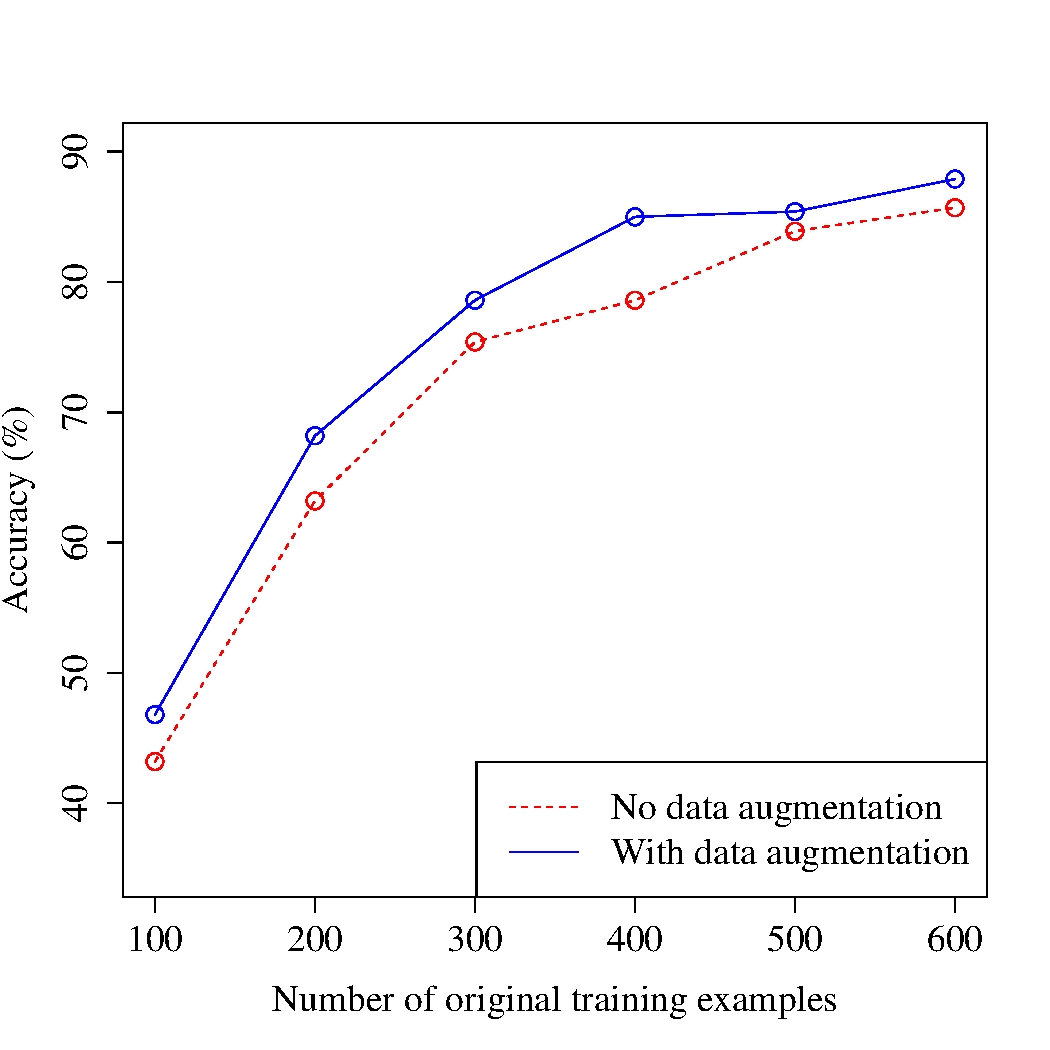
\includegraphics[scale=0.4]{fig-geo-augment.pdf}
\end{center} 
\caption{Accuracy on \geo as a function of number of training examples.
  Data augmentation gives a consistent accuracy boost,
regardless of original dataset size.}
\label{fig:geo-augment}
\end{figure}
\rj{Rewrote quite a bit here, as I think we maybe shouldn't
  focus so much on directly comparing the value of
real and augmented examples, at least in this subsection}

To further measure the effects of compositional data augmentation,
we trained our system both with and without data augmentation
on various random subsets of the \geo dataset.
In Figure~\ref{fig:geo-augment}, we plot test accuracy as a function of
the number of real training examples.
When doing data augmentation on $n$ real examples,
we generated $\frac{n}2$ synthetic examples.

From this plot, we see that data augmentation consistently boosts accuracy,
and that it helps somewhat more when there are fewer real training examples.
In many cases, the augmented examples prove to be
about as helpful as getting new original examples:
test accuracy using $200$ real and $100$ synthetic examples
is nearly that of using $300$ real examples,
and test accuracy using $300$ real and $150$ synthetic examples 
is greater than that of using $400$ real examples.

\subsection{Out-of-Domain Augmentation}
\begin{figure}[t] 
\small
\begin{center} 
  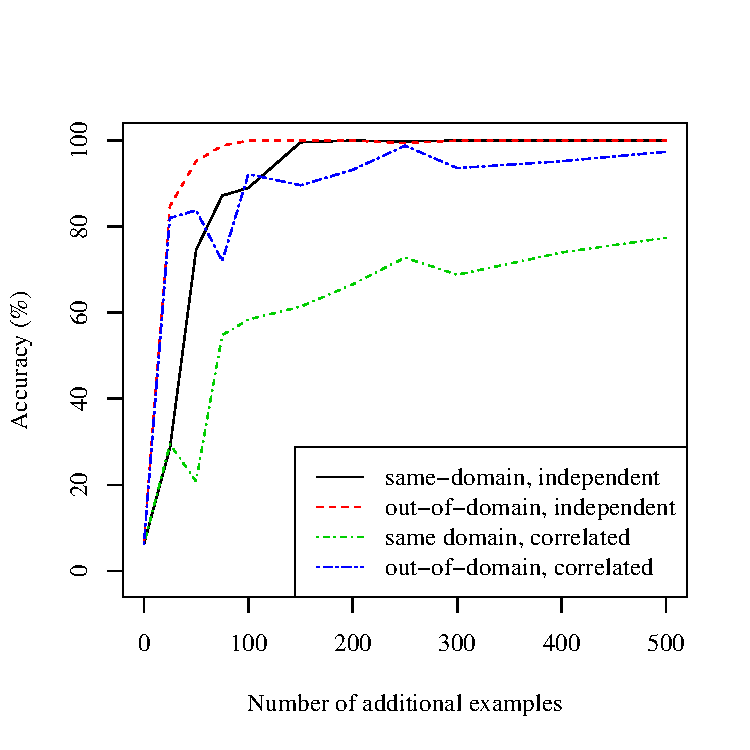
\includegraphics[scale=0.65]{fig-artificial-aug.pdf}
\end{center} 
\caption{Comparing augmentation methods on artificial data.}
\label{fig:artificial}
\end{figure}
% TODO: update this figure for the new experiments

%\begin{table}[t]
%  \centering
%  \small
%  \begin{tabular}{|l|c|}
%    \hline
%    Training Data & Accuracy (on Nested) \\
%    \hline
%    100 Nested (baseline) & $20.2\%$ \\
%    100 Nested + 100 Simple & $91.4\%$ \\
%    100 Nested + 100 Union & $95.0\%$ \\
%    200 Nested & $97.2\%$ \\
%    \hline
%  \end{tabular}
%  \caption{Results of the experiments on artificial data.}
%  \label{tab:artificial}
%\end{table}
Our data augmentation on \geo helped accuracy
even though the generated examples were not guaranteed
to be in the support of the test distribution;
meanwhile, data augmentation on \regex and \atis
proved ineffective, even though 
the generated examples there were to the test examples. 
One possible explanation is that by generating longer examples on
\geo, we biased the model to focus on examples that are similar to the
harder examples in the test set.
However, an interesting alternative explanation is that
data augmentation can be most beneficial when the examples generated
do not match the test distribution.
To investigate the effects of such \emph{out-of-domain} data augmentation,
we conducted additional experiments on artificial data.

We generated artificial examples from a simple grammar.
Each example is a pair of an utterance $x$ and logical form $y$.
Our world contains a set of entities and a set of binary relations on entities.
We generate synthetic examples that involve the 
composition of $n$ relations applied to a single entity.
We refer to the number of relations $n$ as the ``depth'' of the example.
Example $(x, y)$ pairs are given in Figure FIGURE.

With this setup, we seek to understand what types of training examples 
are most helpful to our model.
At first, one might expect that the best examples the model can receive
are iid examples drawn from the test distribution.
However, we hypothesize that it can help to have examples
that are not in the support of the test distribution, 
especially if they are longer than those in the test distribution.
Additionally, we hypothesize that if iid examples cannot be obtained,
then compositional data augmentation, 
which generates examples that are correlated
with the initial training set, can still significantly help generalization.
Furthermore, we expect that an augmentation scheme that generates
longer out-of-domain examples may help more than one that only generates
same-domain examples.

We create artificial experiments to test all of these hypotheses.
We choose to focus on mapping utterances to logical forms of depth $2$,
and evaluate the model after being trained on various datasets.
The model always has a small initial training set of $100$ depth-$2$ examples.
Additionally, we add one of four types of examples to the model:
\begin{itemize}
  \item \textbf{Same-domain, independent}: Randomly chosen depth-$2$ examples.
  \item \textbf{Out-of-domain, independent}: Randomly chosen depth-$4$ examples.
  \item \textbf{Same-domain, correlated}: Take the given training examples
    and swap out entity mentions for different entity mentions.
    This is similar to our augmentation strategy for \regex.
    Note that since the training and testing examples
    are both drawn uniformly at random from the set of all depth-$2$ 
    examples, these generated examples also come from that same distribution,
    though they are correlated with the training examples.
  \item \textbf{Out-of-domain, correlated}: Take the given training examples
    and swap out one entity mention for another complete example.
    Also swap out the entity in the second example for a new entity.
    This is similar to our augmentation strategy for \geo.
\end{itemize}
In Figure \ref{fig:artificial}, we plot the accuracy on a test set 
of $500$ depth-$2$ examples versus the number of additional examples added
of each of these four types.
These results confirm our hypotheses.  
First, independent out-of-domain examples are more efficient
at getting the model to achieve perfect accuracy than independent same-domain examples.
Additionally, both data augmentation strategies proved helpful,
with the out-of-domain strategy the more successful of the two.
\rj{I'm sort of lying when I say "independent" in this section because
  what I'm doing is randomly sampling without replacement,
  as randomly sampling with replacement just seemed silly.
Is there a better way to phrase this?}

%\subsection{Data Augmentation and Covariate Shift}
%\begin{table*}[t]
%  \centering
%  \small
%  \begin{tabular}{|l|c|c|c|}
%    \hline
%    Dataset & Accuracy & Accuracy on Int Examples & Accuracy on String Examples \\
%    \hline
%    Original & $65.0$ & $11/19$ & $54/82$ \\
%    Int-Augmented & $67.0$ & $15/19$ & $52/82$ \\
%    String-Augmented & $65.0$ & $8/19$ & $56/82$\\
%    All Augmented & $79.0$ & $17/19$ & $62/82$ \\
%    \hline
%  \end{tabular}
%  \caption{Performance on \regex using different data augmentation strategies.}
%  \label{tab:regex-shift}
%\end{table*}
%
%We have shown that data augmentation can yield significant improvements
%for our model, as it encourages the model to learn good alignments,
%a simple form of compositionality.  Nonetheless,
%there are also drawbacks to our data augmentation, as it introduces
%covariate shift: certain types of examples are more likely than others
%to occur in our augmented data.
%
%To illustrate the effects of covariate shift, we ran an additional
%experiment on the \regex dataset.  We trained our model
%on the original dataset plus augmented data generated only from the
%integer-based scheme; we also trained a separate copy of the model
%on the original dataset plus augmented data generated only from the
%string-based scheme.  
%
%The results of this experiment are summarized in Table \ref{tab:regex-shift}.
%We see that in isolation, each individual data augmentation scheme
%does not significantly help accuracy.
%The integer-based augmentation helps the model deal better
%with utterances that contain an integer 
%(third column of Table \ref{tab:regex-shift}),
%but hurts performance on other examples.
%Similarly, the string-based augmentation helps the model
%deal better with utterances that contain quoted strings 
%(fourth column of Table \ref{tab:regex-shift}),
%but hurts performance on other examples.
%Pooling both sources of augmented data improves performance
%across the board.

\section{Discussion and Related Work}
\label{sec:discussion}
In this paper, we have presented the first sequence-to-sequence
model for semantic parsing.  Our model is easy to train
and gives good accuracy on several semantic parsing
datasets, when trained with logical form supervision.

% Rare words
Our model includes a novel attention-based copying mechanism
to deal with unseen words such as entity names that are found in many semantic parsing datasets.
Previous work on neural machine translation has also tackled the problem of rare words.
In particular, \newcite{luong2015rare} proposed models for copying unknown
tokens from the input to the output.
Their proposed techniques require preprocessing the dataset
with a separate tool to align words between the input and output,
which we do not need.
Furthermore, during training, their method is only activated when the model
wants to write a rare output word. 
In contrast, our attention-based copying can be used for 
both rare and common words,
so our model can learn when it is best to perform copying.

% Augmentation
Additionally, we describe a compositional data augmentation approach that 
further boosts accuracy.
Data augmentation in general has been shown to help neural networks,
particularly in the field of computer vision.
AlexNet \cite{krizhevsky2012imagenet}, 
which at the time drastically improved
the state-of-art on ImageNet,
was trained on augmented data generated by applying various transformations
to the input images that did not change the output label.
The data augmentation scheme we propose has a more general flavor,
as it is not constrained to keep the output label fixed.
We are able to generate synthetic examples $(x, y)$
where neither $x$ nor $y$ occur in the training dataset.

Interestingly, our experiments on artificial data show that
our data augmentation strategy can help the model learn
even when the new examples look different than the examples seen at test time.  
It is conceivable that these \emph{out-of-domain} synthetic examples
act as a regularizer that encourages the model
to learn good representations of the data.
Much further work is needed to explore the potential of
similar data augmentation techniques in other domains
and for other types of machine learning models.
\pl{too vague}
\pl{cite more broadly:
dropout training \cite{hinton2012improving,wager2014altitude}
knowledge base completion \cite{guu2015traversing}.
}

% Grammar induction
We used a small set of high-precision manual rules to perform data augmentation.
It is possible that an automatic grammar induction approach,
such as that of \newcite{kwiatkowski10ccg},
could expand the recall of our grammar while keeping precision high.

% Denotations
One limitation of our current approach is that it 
uses annotated logical forms as supervision.
In the last few years, there has been an emergence of
semantic parsers that can learn from denotations 
\cite{clarke10world,liang11dcs,berant2013freebase,artzi2013weakly}.
In principle, our system could learn from denotations as well,
but it would need a way to generate valid candidate logical forms
early on during training.

% Executor into network
An alternative direction would be to incorporate the execution
step itself into the network.  \newcite{yin2015enquirer}
explore the idea of having a neural network that maps
SQL queries to denotations.  Such a system could be trained
on natural language queries instead of SQL.
\newcite{bordes2015simple}
who similarly replace a database engine with a memory network
whose memories encode all the relations in the database.
\newcite{guu2015traversing} learns how to execute simple path queries.

%\section*{Acknowledgments}
%Do not number the acknowledgment section.

%\section*{Reproducibility}
%All experiments will be available on Codalab. 

\bibliography{all}
\bibliographystyle{naaclhlt2016}


\end{document}
